% ================= APPENDIX: CAD & CONSTRUCTION =================
\section{CAD and Construction Detail}
\label{app:cad}

This appendix holds the mechanical detail deliberately kept out of
Section~\ref{sec:mechanical}: the model tree, the drawing set, the fabrication
settings and the assembly sequence. The rationale for the architecture --- why
the frame is split, what fixes the envelope, how the wheel is tuned --- stays in
Section~\ref{sec:mechanical} and is not repeated here. Anything in this appendix
may change without the design intent changing; anything in
Section~\ref{sec:mechanical} may not.

\subsection{Design Parameter Table}
\label{app:cad_params}

Table~\ref{tab:cad_params} is the single source of the driving dimensions
referenced by every part in the model, per convention~1 of
Section~\ref{sec:cad_method}. It is the CAD-side mirror of the envelope closure
of Section~\ref{sec:massbudget} and is updated on each iteration. It lists only
what the CAD skeleton drives; the complete set of final values is
Appendix~\ref{app:specs}, and this table is subordinate to it.

\begin{table}[htbp]
\centering
\caption[Driving CAD parameters]{Driving CAD parameters. Every dependent feature
references these; no part carries a duplicated hard-coded value. Released values
are drawn from the specification sheet of Appendix~\ref{app:specs}.}
\label{tab:cad_params}
\small
\setlength{\tabcolsep}{4pt}
\begin{tabular}{l L{4.7cm} c L{4.6cm}}
\toprule
Symbol & Parameter & Value & Status and closure \\
\midrule
$L$         & Cube edge length (outer)                & \qty{\cubeL}{\milli\metre} & Released; frozen at M2a \\
$t_w$       & Frame wall thickness                    & \qty{\cubeWall}{\milli\metre} & Released; frozen with $L$ \\
$D_w$       & Wheel outer diameter (Sec.~\ref{sec:rw_sizing}) & \qty{\wheelOD}{\milli\metre} & Released; set by the envelope closure \\
$t_r$       & Wheel axial thickness (Sec.~\ref{sec:rw_sizing}) & \qty{\wheelT}{\milli\metre} & Released; set by the inertia target \\
\bottomrule
\end{tabular}
\end{table}

\subsection{Model Tree and Part List}
\label{app:cad_tree}

Table~\ref{tab:cad_parts} lists the modelled parts by assembly, with their
fabrication route and current status. It is the mechanical counterpart to the
electronics bill of materials of Appendix~\ref{app:bom}: the parts here are the
team's design responsibility and are not supplied.

\begin{table}[htbp]
\centering
\caption[CAD model tree and part list]{CAD model tree and part list. Quantities are per assembled cube unless
noted; the 1-DoF rig parts are listed separately.}
\label{tab:cad_parts}
\small
\setlength{\tabcolsep}{4pt}
\begin{tabular}{c L{4.0cm} c L{3.4cm} L{3.0cm}}
\toprule
Ref & Part & Qty & Fabrication route & Status \\
\midrule
\multicolumn{5}{@{}l}{\textbf{Inner structure}}\\
\midrule
M1 & Motor subframe             & --- & 3D print & Built \\
M2 & Motor mount ($\times$axis) & 3 & 3D print & Built \\
M3 & Battery cradle / retention & 1 & 3D print & Built \\
M4 & Electronics tray           & 1 & 3D print & Built \\
M5 & Brake servo bracket        & 3 & --- & Not built \\
\midrule
\multicolumn{5}{@{}l}{\textbf{Reaction wheel assembly}}\\
\midrule
W1 & Ballasted ring (Sec.~\ref{sec:rw_sizing}) & 3 & PET-CF 3D print & Built \\
W2 & Wheel hub / rotor adapter  & 3 & PET-CF 3D print & Built \\
W3 & Ballast bolt and nut set (M6, $\wheelN$ per wheel) & 45 & Standard hardware & Built \\
W4 & Brake strike feature       & 3 & --- & Not built \\
\midrule
\multicolumn{5}{@{}l}{\textbf{Outer frame}}\\
\midrule
F1 & Frame member / edge rail   & --- & 3D print & Built \\
F2 & Corner contact feature     & 8 & 3D print & Built \\
F3 & Face panel / wheel guard   & --- & 3D print & Built \\
\midrule
\multicolumn{5}{@{}l}{\textbf{1-DoF rig (Sec.~\ref{sec:cad_2d})}}\\
\midrule
R1 & Face plate                 & 1 & 3D print & Built \\
R2 & Pivot bearing mount        & 1 & 3D print & Built \\
R3 & Rig motor mount            & 1 & 3D print & Built \\
R4 & Hard stops / containment   & 2 & 3D print & Built \\
\bottomrule
\end{tabular}
\end{table}

\subsection{1-DoF Prototype Construction}
\label{app:cad_2d}

% Rig drawings and construction notes: plate geometry, pivot bearing seat,
% motor mount, brake barrier travel, hard-stop placement, and the mounting
% location of the IMU relative to the pivot (Sec.~\ref{sec:imu_mount}).

The general-assembly drawing of the 1-DoF rig is given in
Figure~\ref{fig:dwg_2d}. This is the final released design of the single-axis
prototype: the sheet carries the orthographic set --- front and side elevations
of the rig on its base, and a plan and edge view of the reaction-wheel assembly
--- from which the plate geometry, the pivot bearing seat, the motor bolt circle
and the hard-stop placement are taken. The rig as built from this drawing is
shown in Figure~\ref{fig:rig_2d}.

% The drawing sheet is drawn on its own landscape page rather than scaled into
% the text block: reduced to \textwidth in portrait the views and the title
% block fall below legibility. Same treatment as the full schematic of
% App.~\ref{app:schematic_full} and the Gantt sheets of Sec. 3.
%
% Source: images/1D_2dwg.pdf, a single-page landscape vector export of the
% general-assembly drawing. On a landscape page \linewidth is the long edge, so
% the height limit is expressed in \textwidth -- with keepaspectratio, whichever
% bound binds first is the one applied.

% Empty page style for the rotated sheet: the running header and footer would
% otherwise be typeset sideways along the page edge.
\fancypagestyle{cublidrawing}{%
  \fancyhf{}%
  \renewcommand{\headrulewidth}{0pt}%
  \renewcommand{\footrulewidth}{0pt}%
}

\begin{landscape}
\pagestyle{cublidrawing}
\begin{figure}[p]
\thispagestyle{cublidrawing}
\centering
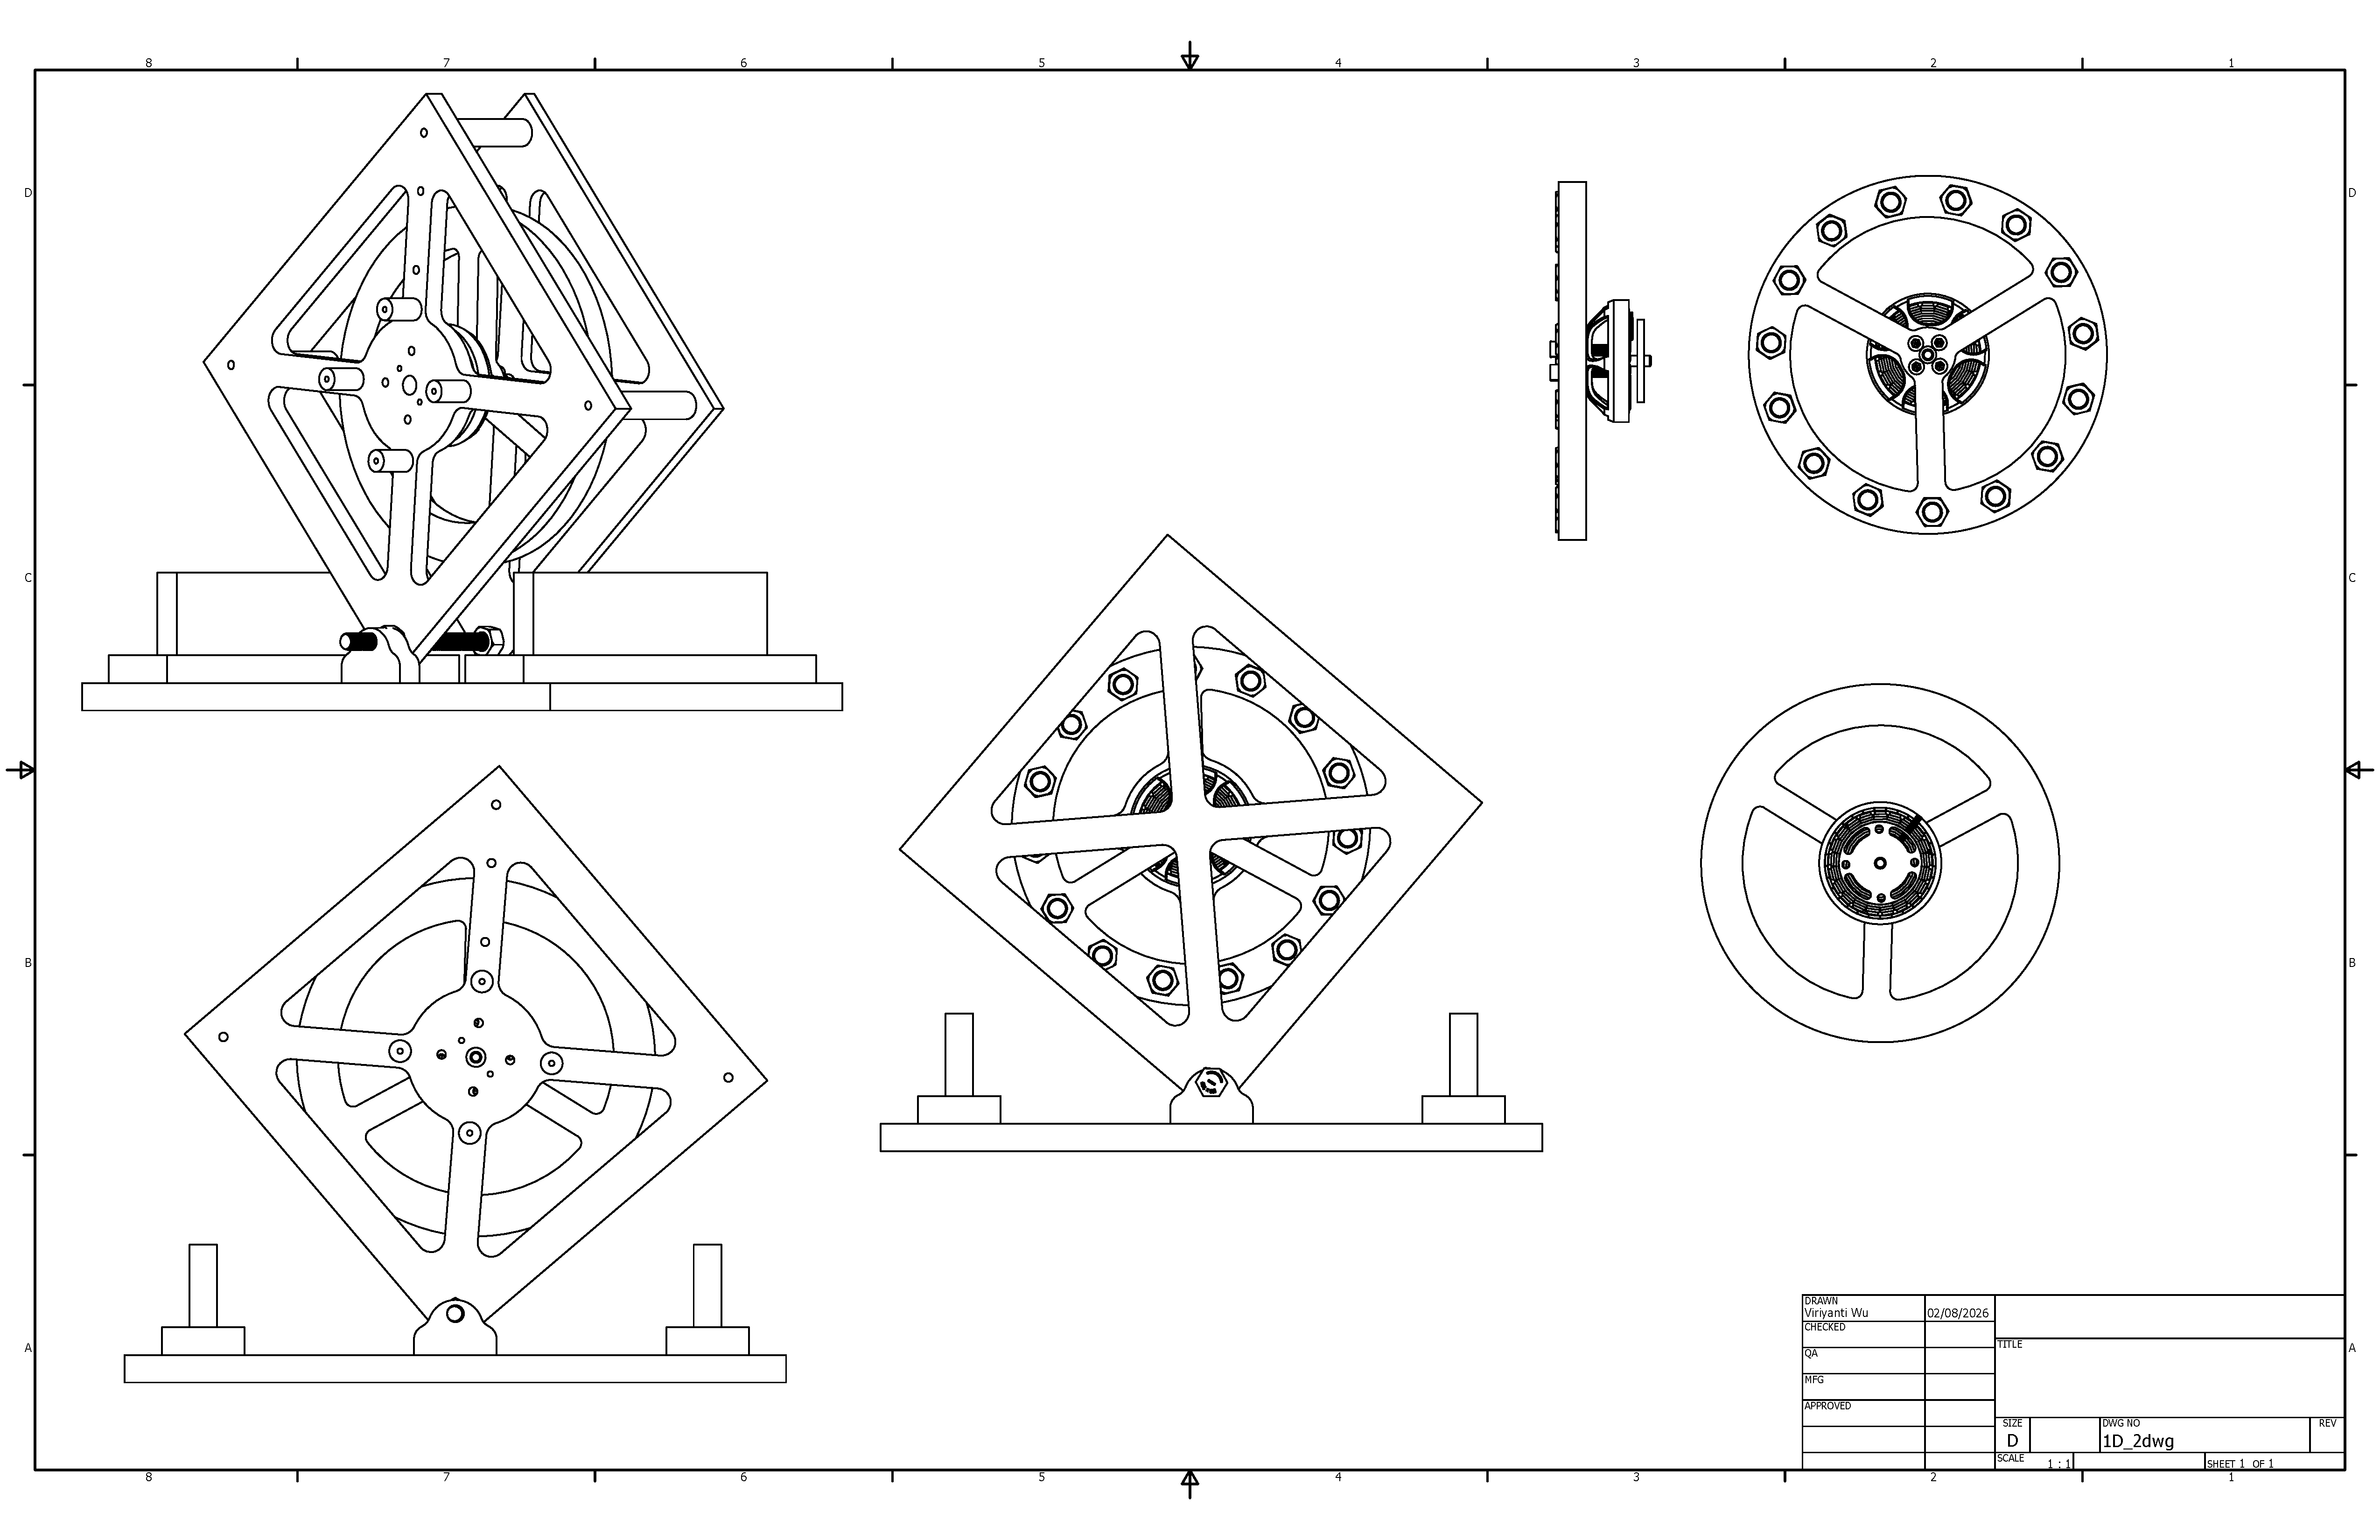
\includegraphics[width=\linewidth,height=1.0\textwidth,keepaspectratio]{images/1D_2dwg.pdf}
\caption[General-assembly drawing of the 1-DoF prototype rig]{General-assembly
drawing of the 1-DoF prototype rig --- the final released design of the
single-axis article --- sheet 1 of 1 at 1:1. Upper left and lower left: front
elevation of the rig mounted on its base, showing the diagonal plate
orientation, the corner pivot and the two hard stops. Centre: side elevation
through the wheel axis. Right: plan and edge views of the reaction-wheel and
motor assembly, giving the spoke pattern and the ballast bolt circle used for
the balancing adjustment of Section~\ref{sec:rw_sizing}.}
\label{fig:dwg_2d}
\end{figure}
\end{landscape}
\pagestyle{fancy}

\subsection{3D Cube Construction}
\label{app:cad_3d}

The general-assembly drawing of the three-axis cube is given in
Figure~\ref{fig:dwg_3d}. The frame realises the two-part architecture of
Section~\ref{sec:mechanical}: an outer frame of edge rails and corner contact
features encloses an inner structure carrying the three orthogonal
reaction-wheel modules and the electronics tray. The sheet carries an isometric
cutaway of the inner structure with the individual boards called out (upper
left), an isometric view of the closed assembly with the three wheel modules
visible through the open frame faces and the ballast bolt set annotated (upper
centre), a front elevation of a single motor/wheel module in section, with the
IMU location called out (right), and two front orthographic views of individual
face modules giving the motor bolt circle and corner fastener pattern (lower
left and centre). This drawing supersedes the concept prototype of
Figure~\ref{fig:cube_3d}, which validated the two-part architecture and internal
packaging but did not carry final dimensions; the edge length $L$ and wheel
geometry realised here follow the closure of Section~\ref{sec:rw_sizing}.

\begin{landscape}
\pagestyle{cublidrawing}
\begin{figure}[p]
\thispagestyle{cublidrawing}
\centering
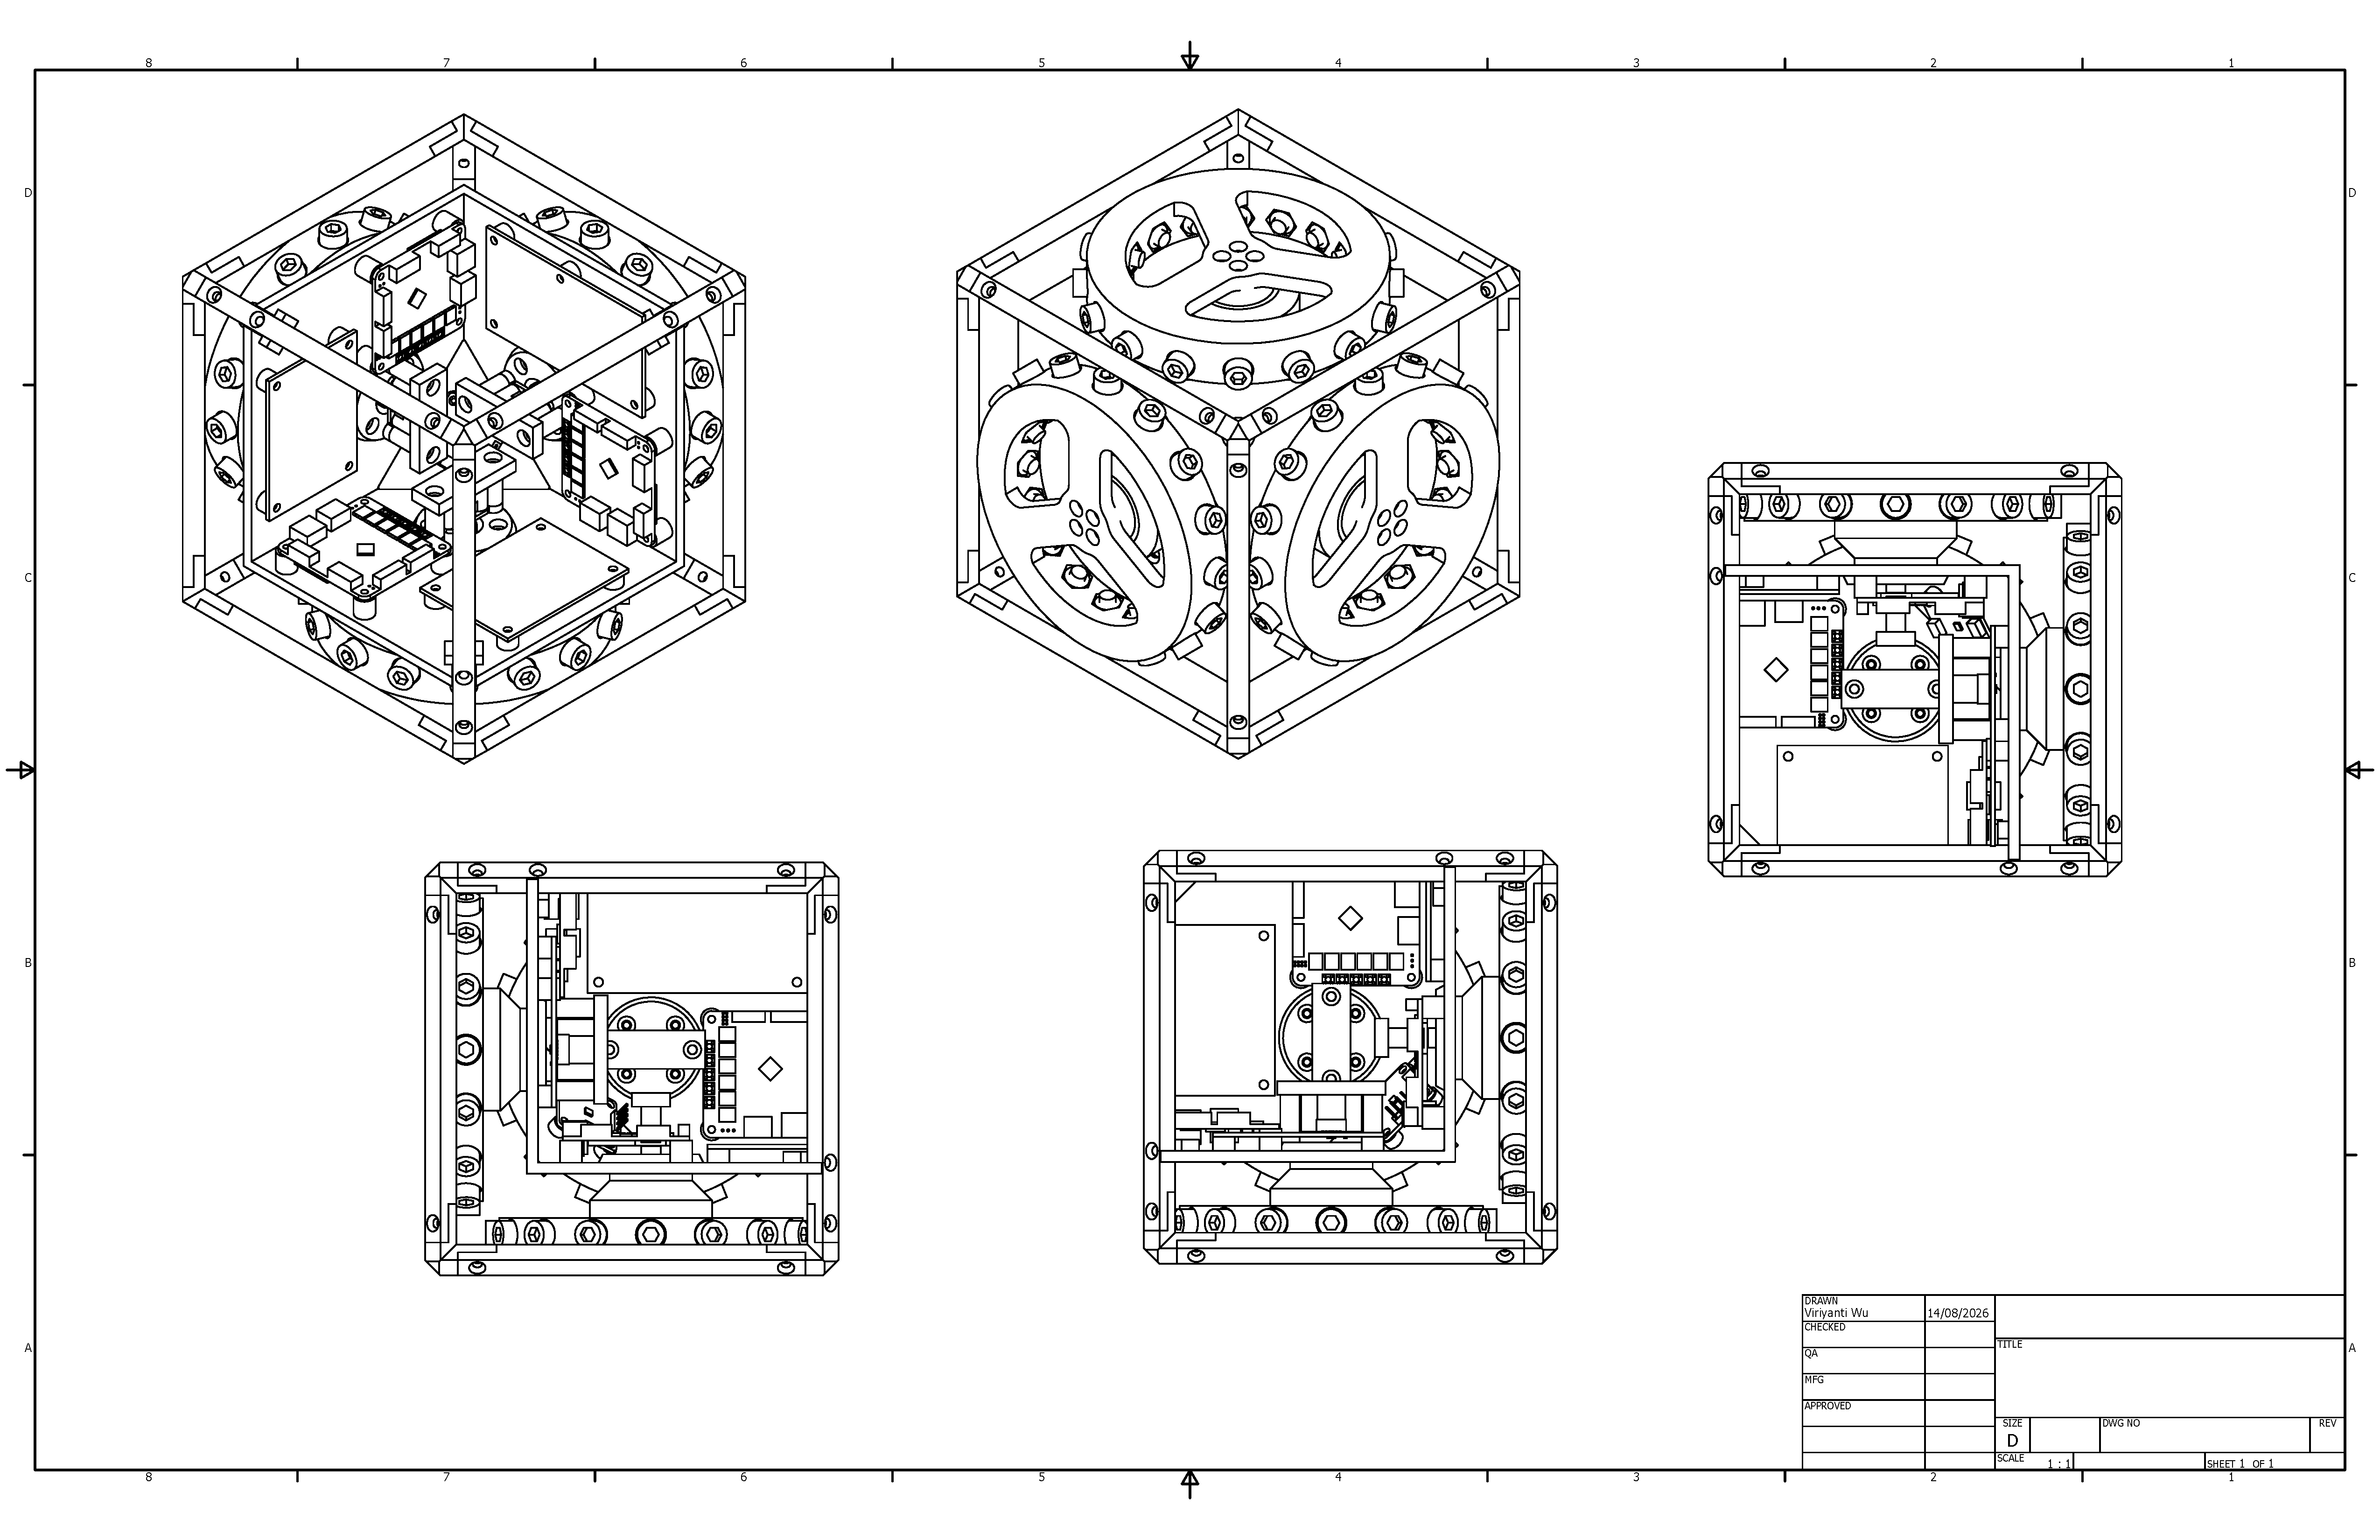
\includegraphics[width=\linewidth,height=1.0\textwidth,keepaspectratio]{images/armonia_assembly.pdf}
\caption[General-assembly drawing of the three-axis cube, with electronics
callouts]{3D visualization of the final three-axis cube flight article. The render highlights the internal structure containing three motor drivers, three encoder boards, and three core perfboards (Teensy FC, Xiao, DC-DC converter), integrated alongside three orthogonal reaction-wheel assemblies, the inner IMU, and frame ballast hardware.}
\label{fig:dwg_3d}
\end{figure}
\end{landscape}
\pagestyle{fancy}

The IMU callout above marks its physical location only: its sensing axes are
not aligned with the body frame $\{B\}$ of Figure~\ref{fig:cubli_3dof}, and the
fixed correction applied in software is given in
Section~\ref{sec:imu_mount}.

\subsection{Fabrication and Assembly}
\label{app:cad_fab}

\subsubsection{Assembly Sequence}

The sequence of Table~\ref{tab:assembly_seq} is ordered by access: each step is
one whose verification becomes impossible or destructive once a later step is
complete. The encoder air gap in particular is re-checked after mechanical
assembly, since it can shift when the structure is bolted up
(Table~\ref{tab:schematic_sheets}).

\begin{table}[htbp]
\centering
\caption[Assembly sequence]{Assembly sequence. Ordering is set by access: each check must be
completed before the step that encloses it.}
\label{tab:assembly_seq}
\small
\begin{tabular}{c L{5.6cm} L{6.4cm}}
\toprule
Step & Operation & Check before proceeding \\
\midrule
1 & Wheel assembly: ring, hub, ballast bolts to the selected count & Balance check; bolt retention per Sec.~\ref{sec:rw_sizing} \\
2 & Motor to mount, encoder magnet to rotor & Encoder air gap and centring to the assembly spec \\
3 & Motor modules to inner structure, three axes & Axis orthogonality; wheel clearance $c_w$, $c_o$ \\
4 & Battery and electronics tray into inner structure & Pack centring; board keep-out clearances \\
5 & Harness install and dressing & Continuity and isolation (Sec.~\ref{sec:electrical_safety}) \\
6 & Inner structure into outer frame & Encoder air gaps re-checked after bolt-up \\
7 & Contact features and guards & Contact geometry; wheel guard clearance \\
8 & Mass properties measurement & Measured mass against Table~\ref{tab:massbudget} \\
\bottomrule
\end{tabular}
\end{table}

\subsection{Mass Properties Verification}
\label{app:cad_mass}

The CAD roll-up is an estimate until the assembly is weighed. Step~8 above
closes the loop of Section~\ref{sec:massbudget}: the measured mass is compared
against the modelled value, and any discrepancy is carried back into
$I_{w,\text{target}}$ and absorbed, where possible, by the ballast trim of
Section~\ref{sec:rw_sizing} rather than by a re-design.

\begin{table}[htbp]
\centering
\caption[Modelled versus measured mass properties]{Modelled versus measured mass properties. A discrepancy here is
absorbed by ballast trim where the margin allows.}
\label{tab:mass_verification}
\small
\begin{tabular}{L{4.6cm} c c c}
\toprule
Quantity & CAD value & Measured & Discrepancy \\
\midrule
Total cube mass $M$          & \qty{\Mbasis}{\kilo\gram}\textsuperscript{*} & \qty{\Mbuilt}{\kilo\gram} & $-$\qty{\Mdelta}{\gram} \\
Wheel mass $m_w$ (each)      & \qty{\wheelMass}{\gram} & --- & --- \\
Wheel inertia $I_w$ (each)   & \qty{\wheelI}{\kilogram\metre\squared} & --- & --- \\
\bottomrule
\end{tabular}

\vspace{0.4em}
{\footnotesize\RaggedRight\textsuperscript{*}\,Not a closed CAD roll-up: the
\qty{1.800}{\kilo\gram} is the budget of Table~\ref{tab:massbudget}, whose
structural line is still an allowance. It is quoted here as the value the
measurement is compared against.\par}
\end{table}

\paragraph{As-built mass, and what the underrun is worth.} The integrated cube
weighs \qty{1.626}{\kilo\gram} --- \qty{174}{\gram} below the
\qty{1.800}{\kilo\gram} sizing basis of Table~\ref{tab:jumpup_budget}, and
inside the \qty{1.8}{\kilo\gram} cap of CON-02. The difference is entirely
structural: the specified hardware of Table~\ref{tab:massbudget} totals
\qty{1367.5}{\gram} and is measured or taken from datasheets, so the realised
structure comes to \qty{258.5}{\gram} against the \qty{432.5}{\gram} allowance
the budget carries.

The sizing basis is deliberately \emph{not} revised to match.
Section~\ref{sec:sizing} sizes against the heaviest mass the design admits
rather than the lightest it achieves, so \qty{1.800}{\kilo\gram} remains the
figure PER-06 is derived at and the wheel is built to. What the underrun
changes is margin, not requirement. Re-evaluating
Equations~\eqref{eq:hw_ideal}--\eqref{eq:Iw_target} at \qty{1.626}{\kilo\gram}
gives $\tau_g = \qty{1.1884}{\newton\metre}$, $\beta = \num{1.3118}$ and $h_w
= \qty{0.2281}{\kilo\gram\metre\squared\per\second}$, hence
$I_{w,\text{target}} = \qty{5.4445e-4}{\kilogram\metre\squared}$: the
fifteen-station wheel delivers \qty{115.2}{\percent} of what the built cube
actually demands, against the \qty{100.6}{\percent} it delivers against the
basis it was sized on. Equivalently, the same wheel closes the corner jump-up
at any speed down to about \qty{3470}{\rpm}, so the \qty{4000}{\rpm} design
point carries some \qty{530}{\rpm} of speed margin on the article as built.
That margin is realised, and is not to be spent by relaxing the sizing basis
or by allowing the structure to grow back into its allowance.
